\documentclass{article}
\usepackage[left=2cm, bottom=2cm,right=2cm,top=2cm]{geometry}
\usepackage[utf8]{inputenc}
\usepackage{amsmath,amsfonts,amssymb,mathtools}
\usepackage{bm}
\usepackage{graphicx}
\usepackage{float}
\usepackage{multirow}
\usepackage{tabularx}
\usepackage{makecell}
\usepackage{caption}
\usepackage{subcaption}
\usepackage{pdflscape}
\graphicspath{ {./images/} }
\usepackage{hyperref}
\usepackage{enumitem}
\usepackage[xindy={glsnumbers=false}, nonumberlist, nopostdot, nogroupskip]{glossaries}

\usepackage{pifont}% http://ctan.org/pkg/pifont
\newcommand{\cmark}{\ding{51}}%
\newcommand{\xmark}{\ding{55}}%

\usepackage{afterpage}
\newcommand\blankpage{%
    \null
    \thispagestyle{empty}%
    \addtocounter{page}{-1}%
    \newpage}

\usepackage{nomencl}

\DeclareMathOperator*{\argminA}{argmin}
\DeclareMathOperator*{\minA}{min}

\title{Image Denoising}
\author{Ted (Yining) Ding\\
\href{mailto:yd2007@hw.ac.uk}{yd2007@hw.ac.uk}}
\date{July 2021}

\begin{document}
\maketitle

This document is a supplement to the following GitHub repository on image denoising: \url{https://github.com/tedyiningding/Image-Denoising}.

\section*{Grayscale image denoising} \label{sec:gray_denoising}
The following two methods of denoising a grayscale image will be investigated: TV denoising and TGV denoising.

\subsection*{TV denoising} \label{sec:tv_denoising}
Consider a grayscale image of size \(M \times N\), Total Variation (TV) denoising (more specifically, we mean the ROF model \cite{rudin1992nonlinear}) finds the unique solution \(x^\star \in \mathbb{R}^{M \times N}\) which minimises\\
%
\[\frac{1}{2} \left\Vert x-y \right\Vert ^2 + \lambda \left\Vert x \right\Vert_{\text{TV}}\]\\
%
where \(y \in \mathbb{R}^{M \times N}\) is the observed image, \(\lambda\) is a regularisation parameter that balances the two terms, and \(\left\Vert \cdot \right\Vert_{\text{TV}}\) is the total variation of an image which is defined by \\
%
\[\left\Vert x \right\Vert_{\text{TV}} = \left\Vert \mathrm{D} x \right\Vert_{p,1} = \sum_{i=1,j=1}^{M,N} \left| \left( \mathrm{D} x \right)_{i,j} \right|_p = \sum_{i=1,j=1}^{M,N} \left( \left( \mathrm{D} x \right)_{i,j,1}^p + \left( \mathrm{D} x \right)_{i,j,2}^p \right)^{1/p}\]\\
%
where \(\mathrm{D}: \mathbb{R}^{M \times N} \rightarrow \mathbb{R}^{M \times N \times 2}\) is the discrete gradient operator. That is, \(\left\Vert \cdot \right\Vert_{\text{TV}}\) is the \(\ell_1\)-norm of the \(p\)-norm of the pixelwise image gradients \cite[pp. 168]{chambolle2016introduction}. When \(p=1\), it is called the anisotropic TV; whereas when \(p=2\), it is called the isotropic TV. The code uses the latter.

The \href{https://github.com/tedyiningding/Image-Denoising/blob/main/TVdenoise.m}{code} solves the aforementioned problem using the over-relaxed Chambolle-Pock algorithm \cite[Algorithm 3.1]{condat2013primal} after obtaining a saddle-point problem \cite[Example 5.6]{chambolle2016introduction}.

\subsection*{TGV denoising} \label{sec:tgv_denoising}
TV regularisation only promotes piecewise constant structures therefore the result could suffer from staircasing artefacts (as will be seen from the denoised images shown below). To combat this, Total Generalised Variation (TGV) was proposed in \cite{bredies2010total}. The second order TGV promotes not only piecewise constant structures, but also piecewise affine structures. Again, consider a grayscale image of size \(M \times N\), TGV denoising finds the unique solution \(u^\star \in \mathbb{R}^{M \times N}\) (and the unique optimiser of an auxiliary variable \(\mathbf{v}^\star = \left( v_{1}^\star, v_{2}^\star \right) \in \mathbb{R}^{M \times N \times 2}\) which minimises \\
%
\[\frac{1}{2} \left\Vert u - y \right\Vert^{2} + \lambda_{0} \left\Vert \mathrm{J}\mathbf{v} \right\Vert_{2,1} + \lambda_{1} \left\Vert \mathrm{D}u - \mathbf{v} \right\Vert_{2,1}\]\\
%
where the discrete gradient operator \(\mathrm{D}\) is the same as in the TV denoising example, the operator \(\mathrm{J}: \mathbb{R}^{M \times N \times 2} \rightarrow \mathbb{R}^{M \times N \times 4}\) can be decomposed into \(\mathrm{J}\mathbf{v} = \left( \mathrm{D} v_1, \mathrm{D} v_2 \right)\) \cite[Sec. 7.2.]{chambolle2016introduction}

As can be seen from the equation above, piecewise affine parts in an image will lead to small values to the last two terms, whereas piecewise constant parts do not.

Similar to the TV Denoising code, the \href{https://github.com/tedyiningding/Image-Denoising/blob/main/TGVdenoise.m}{code} solves the problem using the over-relaxed Chambolle-Pock algorithm \cite[Algorithm 3.1]{condat2013primal} after obtaining a saddle-point problem \cite[Sec. 7.2.]{chambolle2016introduction}.

\subsection*{Results comparison} \label{sec:results_gray}
Qualitative results are shown in Figure \ref{fig:gray_comparison}. We also show some quantitative results including the reconstructed signal-to-noise ratio (RSNR) and the structural similarity index measure (SSIM) in Table \ref{tab:gray_metrics}.
\begin{figure}[htbp]     
    \centering
    \begin{subfigure}[b]{0.24\textwidth}
        \centering
        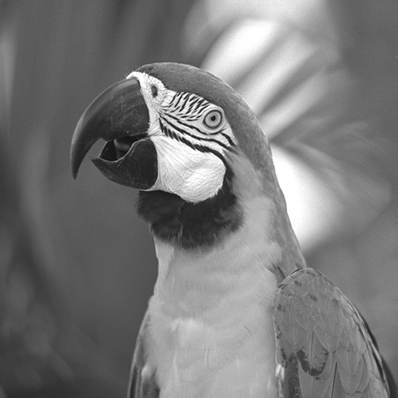
\includegraphics[width=\textwidth]{images/gray.png}
        \caption{The original image}
        \label{fig:gray}
    \end{subfigure}
    \hfill
    \begin{subfigure}[b]{0.24\textwidth}
        \centering
        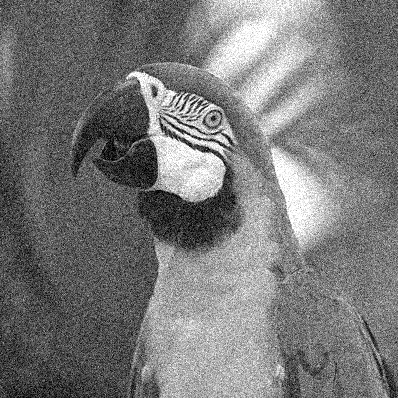
\includegraphics[width=\textwidth]{images/noisy_gray.png}
        \caption{The noisy image}
        \label{fig:noisy_gray}
    \end{subfigure}
    \hfill
    \begin{subfigure}[b]{0.24\textwidth}
        \centering
        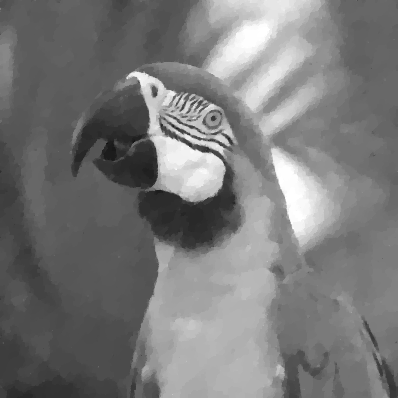
\includegraphics[width=\textwidth]{images/TVdenoised_gray.png}
        \caption{TV denoised image}
        \label{fig:TVdenoised_gray}
    \end{subfigure}
    \hfill
    \begin{subfigure}[b]{0.24\textwidth}
        \centering
        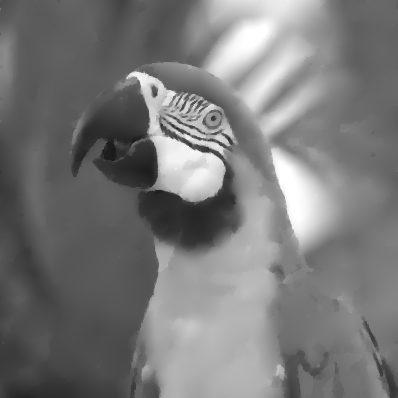
\includegraphics[width=\textwidth]{images/TGVdenoised_gray.png}
        \caption{TGV denoised image}
        \label{fig:TGVdenoised_gray}
    \end{subfigure}
    \vspace{.3cm}

    \caption{Gray image denoising comparison}
    \label{fig:gray_comparison}
\end{figure}

\begin{table}[htbp]
    \centering
    \begin{tabular}{| l | l | l |} 
        \hline
        \textbf{Images} & \textbf{RSNR (dB)} & \textbf{SSIM} \\ [0.5ex] 
        \hline\hline
        Noisy & 14.1727 & 0.1949 \\ 
        \hline
        TV denoised & 25.3879 & 0.8702 \\
        \hline
        TGV denoised & 25.3985 & 0.8859 \\
        \hline
    \end{tabular}
    \caption{Gray image error metrics}
    \label{tab:gray_metrics}
\end{table}

We can see that the TGV method is only marginally higher in RSNR and SSIM but there is no obvious staircasing artefact (see the background).

\section*{Colour image denoising} \label{sec:colour_denoising}
Pixels in a colour image are vector-valued and therefore colour images can be considered as a concatenation of multiple scalar-valued images (i.e. multiple colour channels) in the third dimension. A naive way of denoising a colour image would be to apply techniques for scalar-valued image denoising (e.g. TV denoising) to each colour channel individually, ignoring any coupling between the colour channels. We will investigate some slightly more sophisticated methods.

Now we consider an RGB image \(\mathbf{x}=\left(x_r,x_g,x_b\right) \in \mathbb{R}^{M \times N \times 3}\), where \(x_r,x_g,x_b \in \mathbb{R}^{M \times N}\) represent the three colour channels. Consider a new discrete gradient operator \(\mathbf{D}: \mathbb{R}^{M \times N \times 3} \rightarrow \mathbb{R}^{M \times N \times 2 \times 3}\) such that \(\mathbf{D}\mathbf{x} = \left(\mathrm{D}x_r,\mathrm{D}x_g,\mathrm{D}x_b\right)\), where \(\mathrm{D}\) is the discrete gradient operator for scalar-valued images which we have defined previously in TV denoising. Without loss of generality, we can switch the last two dimensions of \(\mathbf{D}\mathbf{x}\) so now after applying \(\mathbf{D}\), each pixel in \(\mathbf{x}\) corresponds to a matrix of size \(3 \times 2\).

The Schatten \(p\)-norm of a matrix \(A \in \mathbb{R}^{P \times Q}\) is defined by the \(\ell_p\)-norm of the vector consisting of the singular values of \(A\):\\
%
\[\left|A\right|_{\mathcal{S}_p} \coloneqq \left( \sum^{\textbf{min}\{P,Q\}}_{n=1} \sigma_{n}^{p}\left(A\right) \right)^{1/p} \]\\
%
where \(\sigma_{n} \left(A\right)\) is the \(n\)th singular value of \(A\), or equivalently the square root of the \(n\)th eigenvalue of \(A^\top A\) or \(A A^\top\). Three special cases of the Schatten \(p\)-norm are listed below.
\begin{itemize}
    \item \(p=1\): the nuclear norm of matrix (i.e. the sum of its singular values)
    \item \(p=2\): the Frobenius norm of matrix (i.e. the square root of the sum of squares of all of its entries)
    \item \(p=\infty\): the operator or spectral norm of matrix (i.e. its largest singular value)
\end{itemize}

Furthermore, calculating the prox of any Schatten \(p\)-norm of a matrix \(A\) is quite simple:
\begin{enumerate}
    \item Apply SVD to the matrix: \(A = U \Sigma V^\top\)
    \item Extracting the diagonal entries of \(\Sigma\) to make a vector \(\sigma\left(A\right)\)
    \item Calculate the prox of the \(\ell_p\)-norm of \(\sigma\left(A\right)\) and denote the result by \(\hat{\sigma}\left(A\right)\). For example, when \(p=1\), it is the well-known soft-thresholding operator.
    \item The prox of the Schatten \(p\)-norm of a matrix \(A\) is just \(U \  \text{diag}\left(\hat{\sigma}\left(A\right)\right) \  V^\top\)
\end{enumerate}

\subsection*{TNV denoising} \label{sec:tnv_denoising}
From the explanations above we can already see that the Total Nuclear Variation (TNV) denoising (i.e. \(p=1\)) forces every matrix corresponding to a pixel in a vector-valued image to be of low rank (i.e. suppress small non-zero singular values to zeros and shrinks big non-zeros ones). More concretely, it finds the unique solution \(\mathbf{x}^\star \in \mathbb{R}^{M \times N \times 3}\) which minimises\\
%
\[\frac{1}{2} \left\Vert \mathbf{x}-\mathbf{y} \right\Vert ^2 + \lambda \left\Vert \mathbf{D}\mathbf{x} \right\Vert_{\mathcal{S}_1,1}\]\\
%
Again, the \href{https://github.com/tedyiningding/Image-Denoising/blob/main/TNVdenoise.m}{code} solves the problem using the over-relaxed Chambolle-Pock algorithm \cite[Algorithm 3.1]{condat2013primal} after obtaining a saddle-point problem \cite[Sec. 7.3.]{chambolle2016introduction}.

Because the convex conjugate of a norm is the indicator function of a ball based on the dual norm \cite[Sec. 6.5]{parikh2014proximal}, one will need to calculate the projection of \(A\) onto the Schatten \(\infty\)-norm ball with radius \(\lambda\) when solving the saddle-point problem, which requires an SVD of \(A\) associated with each pixel, or equivalently an eigenvalue decomposition of \(A^{\top}A\) associated with each pixel. Thankfully, when \(A \in \mathbb{R}^{3 \times 2}\), its SVD has a closed-form solution, allowing not only efficient calculations of the projection, but also efficient evaluations of the nuclear norm of \(A\). This can be achieved by first parameterising the orthogonal matrix \(V \in \mathbb{R}^{2 \times 2}\) by an angle \(\theta\):\\
%
\[\begin{bmatrix}
\cos \theta & \sin \theta\\
-\sin \theta & \cos \theta
\end{bmatrix}\]

Please refer to this \href{https://sites.ualberta.ca/~mlipsett/ENGM541/Readings/svd_ellis.pdf}{tutorial} for steps of solving \(\theta\) and the two singular values (\(\sigma_1\) and \(\sigma_2\)) of \(A\). Next, we show how to efficiently solve the projection of \(A\) onto the Schatten \(\infty\)-norm ball with radius \(\lambda\).

It is easy to see that the columns of \(A V\) have norms \(\sigma_1\) and \(\sigma_2\) respectively:\\
%
\[A V = U \Sigma =
\begin{bmatrix}
    \vert & \vert & \vert \\
    u_1   & u_2  & u_3  \\
    \vert & \vert & \vert
\end{bmatrix}
\begin{bmatrix}
    \sigma_1 & 0 \\
    0 & \sigma_2  \\
    0 & 0
\end{bmatrix} = 
\begin{bmatrix}
    \vert & \vert \\
    \sigma_1 u_1   & \sigma_2 u_2  \\
    \vert & \vert
\end{bmatrix}\]\\

Furthermore, because both \(U\) and \(V\) are orthogonal matrices, they preserve matrix norms. Therefore, we can perform the projection on the norm of the two columns. When \(p=\infty\), it amounts to the following element-wise operation:\\
%
\[\hat{\sigma} = \text{min}\{\sigma,\lambda\}\]

Therefore, we just need to rescale each column's norm\\
%
\[\hat{A} V =
\begin{bmatrix}
    \vert & \vert \\
    \hat{\sigma}_1 u_1   & \hat{\sigma}_2 u_2  \\
    \vert & \vert
\end{bmatrix}\]

And therefore\\
%
\[\hat{A} =
\begin{bmatrix}
    \vert & \vert \\
    \hat{\sigma}_1 u_1   & \hat{\sigma}_2 u_2  \\
    \vert & \vert
\end{bmatrix}
V^\top\]

\subsection*{Results comparison} \label{sec:results_colour}
Qualitative results are shown in Figure \ref{fig:colour_comparison}. We also show the RSNR results in Table \ref{tab:colour_metrics}.

\begin{figure}[ht]     
    \centering
    \begin{subfigure}[b]{0.24\textwidth}
        \centering
        \includegraphics[width=\textwidth]{images/colour.png}
        \caption{The original image}
        \label{fig:colour}
    \end{subfigure}
    %\hfill
    \begin{subfigure}[b]{0.24\textwidth}
        \centering
        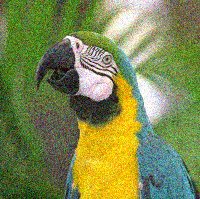
\includegraphics[width=\textwidth]{images/noisy_colour.png}
        \caption{The noisy image}
        \label{fig:noisy_colour}
    \end{subfigure}
    \vspace{.3cm}
    
    \begin{subfigure}[b]{0.24\textwidth}
        \centering
        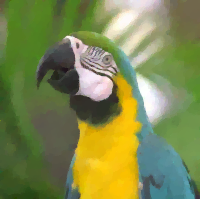
\includegraphics[width=\textwidth]{images/TNVdenoised_colour.png}
        \caption{TNV denoised}
        \label{fig:TNVdenoised_colour}
    \end{subfigure}
    %\hfill
    \begin{subfigure}[b]{0.24\textwidth}
        \centering
        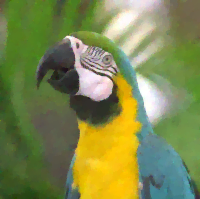
\includegraphics[width=\textwidth]{images/FrobeniusNormdenoised_colour.png}
        \caption{Frobenius norm denoised}
        \label{fig:FrobeniusNormdenoised_colour}
    \end{subfigure}
    %\hfill
    \begin{subfigure}[b]{0.24\textwidth}
        \centering
        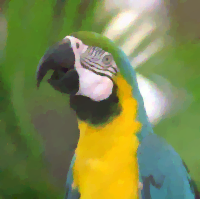
\includegraphics[width=\textwidth]{images/ChannelwiseTVdenoised_colour.png}
        \caption{Channel-wise TV denoised}
        \label{fig:ChannelwiseTVdenoised_colour}
    \end{subfigure}
    \vspace{.3cm}

    \caption{Colour image denoising comparison}
    \label{fig:colour_comparison}
\end{figure}

\begin{table}[ht]
    \centering
    \begin{tabular}{| l | l | l |} 
        \hline
        \textbf{Images} & \textbf{RSNR (dB)} \\ [0.5ex] 
        \hline\hline
        Noisy & 14.1294 \\ 
        \hline
        TNV denoised & 24.3723 \\
        \hline
        Frobenius norm denoised & 24.1266 \\
        \hline
        Channel-wise TV denoised & 23.0542 \\
        \hline
    \end{tabular}
    \caption{Colour image error metrics}
    \label{tab:colour_metrics}
\end{table}

We can see that the TNV denoised has the highest RSNR, which is slightly higher than the one denoised by Frobenius norm. Channel-wise applying TV denoising without considering any coupling between the channels gives the lowest RSNR. In Figure \ref{fig:colour_comparison_zoomed} we show a close-up comparison on a patch of the image with detailed textures.

\begin{figure}[ht]     
    \centering
    \begin{subfigure}[b]{0.24\textwidth}
        \centering
        \includegraphics[scale=2.5,trim={80 117 78 45},clip=true]{images/colour.png}
        \caption{The original image}
        \label{fig:Zoomedcolour}
    \end{subfigure}
    %\hfill
    \begin{subfigure}[b]{0.24\textwidth}
        \centering
        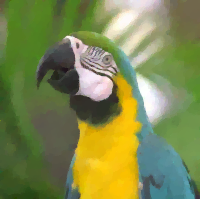
\includegraphics[scale=2.5,trim={80 117 78 45},clip=true]{images/TNVdenoised_colour.png}
        \caption{TNV denoised}
        \label{fig:ZoomedTNVdenoised_colour}
    \end{subfigure}
    %\hfill
    \begin{subfigure}[b]{0.24\textwidth}
        \centering
        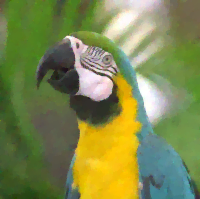
\includegraphics[scale=2.5,trim={80 117 78 45},clip=true]{images/FrobeniusNormdenoised_colour.png}
        \caption{Frobenius norm denoised}
        \label{fig:ZoomedFrobeniusNormdenoised_colour}
    \end{subfigure}
    %\hfill
    \begin{subfigure}[b]{0.24\textwidth}
        \centering
        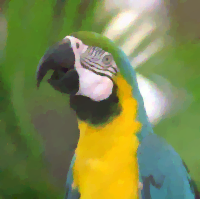
\includegraphics[scale=2.5,trim={80 117 78 45},clip=true]{images/ChannelwiseTVdenoised_colour.png}
        \caption{Channel-wise TV denoised}
        \label{fig:ZoomedChannelwiseTVdenoised_colour}
    \end{subfigure}
    \vspace{.3cm}

    \caption{Colour image denoising detailed comparison}
    \label{fig:colour_comparison_zoomed}
\end{figure}


\bibliographystyle{ieeetr}
\bibliography{bib} \label{bib}

\end{document}
